\documentclass[tikz,border=10pt]{standalone}
\usepackage{amsmath}
\usepackage{tikz}
\usetikzlibrary{arrows.meta, positioning, calc, shapes.geometric}

\begin{document}
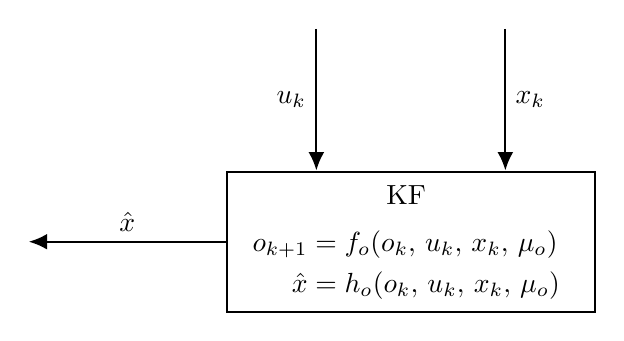
\begin{tikzpicture}[
  block/.style = {draw, thick, minimum height=3em, minimum width=6em, align=center},
  arrow/.style = {thick, -{Latex[width=2mm]}},
  node distance=2.5cm and 2.5cm
]

% KF Block
\node[block] (siggen) {
  \begin{tabular}{c}
    KF \\[0.5em]
    $
    \begin{aligned}
      o_{k+1} &= f_o(o_k,\,u_k,\,x_k,\,\mu_o) \\
      \hat{x} &= h_o(o_k,\,u_k,\,x_k,\,\mu_o)
    \end{aligned}
    $
  \end{tabular}
};

% Top input: u_k (slightly left)
\draw[arrow] ($(siggen.north)+(-1.2,1.8)$) --
  node[midway, left] {$u_k$} ($(siggen.north)+(-1.2,0)$);

% Top input: x_k (slightly right)
\draw[arrow] ($(siggen.north)+(1.2,1.8)$) --
  node[midway, right] {$x_k$} ($(siggen.north)+(1.2,0)$);

% West output going left: \hat{x}
\draw[arrow] (siggen.west) --
  node[midway, above] {$\hat{x}$} ++(-2.5,0);

\end{tikzpicture}
\end{document}
